\documentclass[11pt]{article}
\usepackage[margin=1in]{geometry}
\usepackage{amsmath,booktabs,graphicx}
\graphicspath{{../figures/}{figures/}}
\title{Simulating Mechanical Energy Transfer in Rowing\\\large A Simplified One-Dimensional Model}
\author{Gabriel Cirker}
\date{}
\begin{document}\maketitle
\begin{abstract}
This paper uses a simple model to examine how periodic thrust and quadratic drag affect a rowing shell's speed. A prescribed square-wave force accelerates a single mass during the drive and vanishes during recovery. The results illustrate speed fluctuations and energy accounting during a 20-second startup. The calculation does not measure rower efficiency or validate performance against experimental data.
\end{abstract}
\section{Model}
The boat and crew are represented by a single mass $m$ with speed $v$. The equation of motion is
\begin{equation}m\frac{dv}{dt}=F(t)-kv^2.\end{equation}
For the baseline, $m=766.5$ kg, $k=40$ kg/m, and the prescribed thrust is 3000 N for 0.9 seconds in each 2-second cycle, followed by zero thrust. The boat starts from rest. These values are illustrative model inputs, not measurements from a crew.

The model calculates thrust work $W=\int Fv\,dt$, drag work $D=\int kv^3\,dt$ and the change in kinetic energy $\Delta K=m(v_f^2-v_0^2)/2$. In the continuous model $W-D=\Delta K$. Thrust work on the modeled mass is not the rowers' total mechanical or metabolic work. The ratio $\Delta K/W$ describes how much input work remains as kinetic energy at the end of this startup interval; it is not rowing efficiency and depends on the interval chosen.
\section{Method and results}
The equation is integrated with explicit Euler steps of 0.01 seconds for 20 seconds. The baseline average speed over the latter half is 5.785 m/s and the maximum is 6.759 m/s. Thrust work is approximately 141.2 kJ, drag work 132.3 kJ and kinetic energy gain 9.17 kJ. The gain is 6.49\% of thrust work. The difference of about $-316$ J in $W-D-\Delta K$ is a numerical residual from the discrete scheme.

At a 0.005-second step the residual is about $-158$ J; at 0.001 seconds it is about $-31$ J. The corresponding latter-half average speeds are 5.782 and 5.781 m/s. This convergence check addresses discretization, not the physical accuracy of the inputs.
\begin{figure}[ht]\centering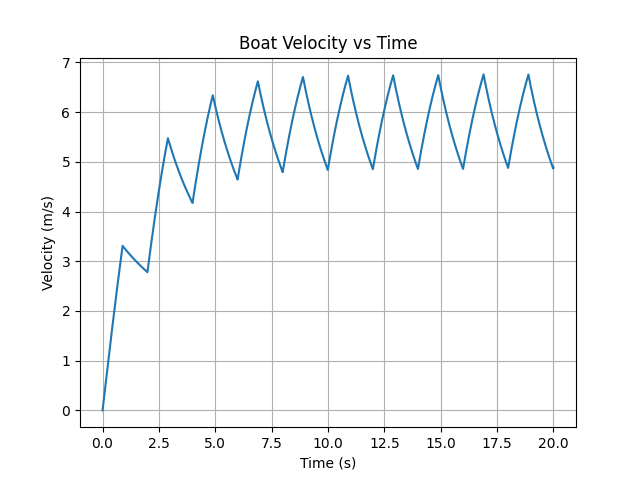
\includegraphics[width=.8\textwidth]{speed_plot.png}\caption{Baseline speed during the 20-second simulation.}\end{figure}
\section{Parameter comparisons and limitations}
With the default step, halving drag raises the latter-half average speed to 8.162 m/s; halving mass gives 5.719 m/s over the same finite interval. Shortening the cycle from 2.0 to 1.5 seconds gives 6.673 m/s, but keeping the drive at 0.9 seconds also increases the drive fraction and input. This is therefore not an isolated comparison at constant work or power.

The model excludes blade slip, rower motion relative to the shell, varying force profiles, wind and waves. It has not been calibrated or compared with measured trajectories. More realistic thrust and drag measurements, timestep checks and experimental validation would be needed before applying the numerical predictions to a crew.
\end{document}
